% Options for packages loaded elsewhere
\PassOptionsToPackage{unicode}{hyperref}
\PassOptionsToPackage{hyphens}{url}
\PassOptionsToPackage{dvipsnames,svgnames,x11names}{xcolor}
%
\documentclass[
  9pt,
  twocolumn,
  twoside]{pnas-new}

\usepackage{amsmath,amssymb}
\usepackage{iftex}
\ifPDFTeX
  \usepackage[T1]{fontenc}
  \usepackage[utf8]{inputenc}
  \usepackage{textcomp} % provide euro and other symbols
\else % if luatex or xetex
  \usepackage{unicode-math}
  \defaultfontfeatures{Scale=MatchLowercase}
  \defaultfontfeatures[\rmfamily]{Ligatures=TeX,Scale=1}
\fi
\usepackage{lmodern}
\ifPDFTeX\else  
    % xetex/luatex font selection
\fi
% Use upquote if available, for straight quotes in verbatim environments
\IfFileExists{upquote.sty}{\usepackage{upquote}}{}
\IfFileExists{microtype.sty}{% use microtype if available
  \usepackage[]{microtype}
  \UseMicrotypeSet[protrusion]{basicmath} % disable protrusion for tt fonts
}{}
\makeatletter
\@ifundefined{KOMAClassName}{% if non-KOMA class
  \IfFileExists{parskip.sty}{%
    \usepackage{parskip}
  }{% else
    \setlength{\parindent}{0pt}
    \setlength{\parskip}{6pt plus 2pt minus 1pt}}
}{% if KOMA class
  \KOMAoptions{parskip=half}}
\makeatother
\usepackage{xcolor}
\setlength{\emergencystretch}{3em} % prevent overfull lines
\setcounter{secnumdepth}{-\maxdimen} % remove section numbering
% Make \paragraph and \subparagraph free-standing
\ifx\paragraph\undefined\else
  \let\oldparagraph\paragraph
  \renewcommand{\paragraph}[1]{\oldparagraph{#1}\mbox{}}
\fi
\ifx\subparagraph\undefined\else
  \let\oldsubparagraph\subparagraph
  \renewcommand{\subparagraph}[1]{\oldsubparagraph{#1}\mbox{}}
\fi


\providecommand{\tightlist}{%
  \setlength{\itemsep}{0pt}\setlength{\parskip}{0pt}}\usepackage{longtable,booktabs,array}
\usepackage{calc} % for calculating minipage widths
% Correct order of tables after \paragraph or \subparagraph
\usepackage{etoolbox}
\makeatletter
\patchcmd\longtable{\par}{\if@noskipsec\mbox{}\fi\par}{}{}
\makeatother
% Allow footnotes in longtable head/foot
\IfFileExists{footnotehyper.sty}{\usepackage{footnotehyper}}{\usepackage{footnote}}
\makesavenoteenv{longtable}
\usepackage{graphicx}
\makeatletter
\def\maxwidth{\ifdim\Gin@nat@width>\linewidth\linewidth\else\Gin@nat@width\fi}
\def\maxheight{\ifdim\Gin@nat@height>\textheight\textheight\else\Gin@nat@height\fi}
\makeatother
% Scale images if necessary, so that they will not overflow the page
% margins by default, and it is still possible to overwrite the defaults
% using explicit options in \includegraphics[width, height, ...]{}
\setkeys{Gin}{width=\maxwidth,height=\maxheight,keepaspectratio}
% Set default figure placement to htbp
\makeatletter
\def\fps@figure{htbp}
\makeatother
% definitions for citeproc citations
\NewDocumentCommand\citeproctext{}{}
\NewDocumentCommand\citeproc{mm}{%
  \begingroup\def\citeproctext{#2}\cite{#1}\endgroup}
\makeatletter
 % allow citations to break across lines
 \let\@cite@ofmt\@firstofone
 % avoid brackets around text for \cite:
 \def\@biblabel#1{}
 \def\@cite#1#2{{#1\if@tempswa , #2\fi}}
\makeatother
\newlength{\cslhangindent}
\setlength{\cslhangindent}{1.5em}
\newlength{\csllabelwidth}
\setlength{\csllabelwidth}{3em}
\newenvironment{CSLReferences}[2] % #1 hanging-indent, #2 entry-spacing
 {\begin{list}{}{%
  \setlength{\itemindent}{0pt}
  \setlength{\leftmargin}{0pt}
  \setlength{\parsep}{0pt}
  % turn on hanging indent if param 1 is 1
  \ifodd #1
   \setlength{\leftmargin}{\cslhangindent}
   \setlength{\itemindent}{-1\cslhangindent}
  \fi
  % set entry spacing
  \setlength{\itemsep}{#2\baselineskip}}}
 {\end{list}}
\usepackage{calc}
\newcommand{\CSLBlock}[1]{\hfill\break\parbox[t]{\linewidth}{\strut\ignorespaces#1\strut}}
\newcommand{\CSLLeftMargin}[1]{\parbox[t]{\csllabelwidth}{\strut#1\strut}}
\newcommand{\CSLRightInline}[1]{\parbox[t]{\linewidth - \csllabelwidth}{\strut#1\strut}}
\newcommand{\CSLIndent}[1]{\hspace{\cslhangindent}#1}

% TODO: Add custom LaTeX header directives here
\makeatletter
\@ifpackageloaded{caption}{}{\usepackage{caption}}
\AtBeginDocument{%
\ifdefined\contentsname
  \renewcommand*\contentsname{Table of contents}
\else
  \newcommand\contentsname{Table of contents}
\fi
\ifdefined\listfigurename
  \renewcommand*\listfigurename{List of Figures}
\else
  \newcommand\listfigurename{List of Figures}
\fi
\ifdefined\listtablename
  \renewcommand*\listtablename{List of Tables}
\else
  \newcommand\listtablename{List of Tables}
\fi
\ifdefined\figurename
  \renewcommand*\figurename{Figure}
\else
  \newcommand\figurename{Figure}
\fi
\ifdefined\tablename
  \renewcommand*\tablename{Table}
\else
  \newcommand\tablename{Table}
\fi
}
\@ifpackageloaded{float}{}{\usepackage{float}}
\floatstyle{ruled}
\@ifundefined{c@chapter}{\newfloat{codelisting}{h}{lop}}{\newfloat{codelisting}{h}{lop}[chapter]}
\floatname{codelisting}{Listing}
\newcommand*\listoflistings{\listof{codelisting}{List of Listings}}
\makeatother
\makeatletter
\makeatother
\makeatletter
\@ifpackageloaded{caption}{}{\usepackage{caption}}
\@ifpackageloaded{subcaption}{}{\usepackage{subcaption}}
\makeatother
\ifLuaTeX
  \usepackage{selnolig}  % disable illegal ligatures
\fi
\usepackage{bookmark}

\IfFileExists{xurl.sty}{\usepackage{xurl}}{} % add URL line breaks if available
\urlstyle{same} % disable monospaced font for URLs
\hypersetup{
  pdftitle={Diverse Genotype-by-Weather Interactions in Switchgrass},
  pdfauthor={Alice H. MacQueen; Li Zhang; Samuel A. Smith; Jason Bonnette; Arvid R. Boe; Phillip A. Fay; Felix B. Fritschi; David B. Lowry; Robert B. Mitchell; Francis M. Rouquette Jr; Yanqi Wu; Arbel Harpak; Thomas E. Juenger},
  pdfkeywords={allele-by-environment effect variation, rank-changing
genotype-by-environment interaction, photoperiod, cumulative
rainfall, genetic variation},
  colorlinks=true,
  linkcolor={blue},
  filecolor={Maroon},
  citecolor={Blue},
  urlcolor={Blue},
  pdfcreator={LaTeX via pandoc}}

\templatetype{pnasresearcharticle}

\title{Diverse Genotype-by-Weather Interactions in Switchgrass}

\newcommand{\equalcont}{1}

\newcommand{\correspond}{2}

\author[a%
,\equalcont%
,\correspond%
]{Alice H. MacQueen}
\author[a%
,\equalcont%
%
]{Li Zhang}
\author[a%
,\equalcont%
%
]{Samuel A. Smith}
\author[a%
%
%
]{Jason Bonnette}
\author[b%
%
%
]{Arvid R. Boe}
\author[c%
%
%
]{Phillip A. Fay}
\author[d%
%
%
]{Felix B. Fritschi}
\author[e%
%
%
]{David B. Lowry}
\author[f%
%
%
]{Robert B. Mitchell}
\author[g%
%
%
]{Francis M. Rouquette Jr}
\author[h%
%
%
]{Yanqi Wu}
\author[a%
%
%
]{Arbel Harpak}
\author[a%
%
,\correspond%
]{Thomas E. Juenger}

\affil[a]{University of Texas at Austin, Department of Integrative
Biology, Austin, 78712}
\affil[b]{South Dakota State University, Department of
Agronomy, Brookings, 57006}
\affil[c]{USDA-ARS, Grassland, Soil and Water Research
Laboratory, Temple, 76502}
\affil[d]{University of Missouri, Division of Plant
Sciences, Columbia, 65211}
\affil[e]{Michigan State University, Department of Plant Biology, East
Lansing, 48824}
\affil[f]{USDA-ARS, Wheat, Sorghum, and Forage Research
Unit, Lincoln, 68583}
\affil[g]{Texas A\&M University, Texas A\&M AgriLife Research and
Extension Center, Overton, 75684}
\affil[h]{Oklahoma State University, Department of Plant and Soil
Sciences, Stillwater, 74078}

\leadauthor{MacQueen}

\significancestatement{The timing of plant seasonal development
(phenology) has major impacts on fitness because of the steep fitness
cost of plant-environment mismatches. We infer the mixture of ways that
genetic effects on phenological traits depend on plant environment,
focusing on how effects covary with weather prior to the phenological
event (GxWeather). Most effects do not have GxWeather, but a minority
do. GxWeather is population-specific. The majority of effects on the
timing of vegetative growth in the Gulf population have GxWeather: these
effects differ in sign across environments and covary with a photoperiod
cue two weeks prior. A minority of effects on flowering date in the Gulf
and Midwest populations had GxWeather, covarying with a cumulative
rainfall and a photoperiod cue, respectively.}

\authorcontributions{T.E.J. designed research. D.B.L. contributed plant
material and resources. J.B., D.B.L., and T.E.J. designed and executed
field experiments. A.R.B., P.A.F., F.B.F., D.B.L., R.B.M., F.M.R., Y.W.,
and T.E.J. hosted field experiments. A.H.M., L.Z., and S.A.S. conducted
statistical and computational analyses. The manuscript was written by
A.H.M. with contributions from all authors.}

\authordeclaration{The authors declare no conflicts of interest.}

\equalauthors{\textsuperscript{\equalcont} A.H.M. contributed equally to
this work with L.Z. and S.A.S.}

\correspondingauthor{\textsuperscript{\correspond}To whom correspondence should be addressed. E-mail: alicem@uchicago.edu}
\correspondingauthor{\textsuperscript{\correspond}To whom correspondence should be addressed. E-mail: tjuenger@utexas.edu}

\keywords{allele-by-environment effect variation | rank-changing
genotype-by-environment interaction | photoperiod | cumulative
rainfall | genetic variation}

\begin{document}
\maketitle

\begin{abstract}
The timing of vegetative and reproductive growth in plants
(``phenological timings'') depends on genetic effects, environmental
(e.g., weather) cues, and possibly their interaction. Quantifying these
GxWeather interactions can aid prediction and manipulation of
phenological timings. Here, we map GxWeather effects on phenological
timings in two highly divergent switchgrass (\emph{Panicum virgatum})
populations using repeated plantings of cloned individuals from these
populations at eight sites across the central United States. Some
genetic effects covary with interpretable weather-based cues. For
example, in the Gulf population, 65\% of genetic effects on the timing
of vegetative growth covary with daylength 14 days prior to green-up
date, and 33\% of genetic effects on the timing of flowering covary with
cumulative rainfall in the seven days prior to flowering. However, most
variation in genetic effects is site-specific and can not be attributed
to variation in the studied weather variables. We demonstrate that we
can identify genetic variation with GxWeather and assign these loci to
specific weather-based cues or other patterns. Breeding for particular
alleles at the GxWeather loci we identified could change flowering
responsiveness in a photoperiod or rainfall-specific way. More broadly,
our approach proposes a refined, powerful characterization of
genotype-by-environment interactions in any species phenotyped in
multiple environments.
\end{abstract}

\dates{This manuscript was compiled on \today}
\doi{\url{www.pnas.org/cgi/doi/10.1073/pnas.XXXXXXXXXX}}

\thispagestyle{firststyle}
\ifthenelse{\boolean{shortarticle}}{\ifthenelse{\boolean{singlecolumn}}{\abscontentformatted}{\abscontent}}{}
\firstpage[17]{2}

Plant phenological timings are major components of plant fitness
affected by multiple external environmental cues (e.g.~degree of winter
chilling, day length, temperature, and water availability) that signal
existing or upcoming growing conditions (1--3). Genetic responses to
environmental cues determine the speed, timing, and energy apportioned
to vegetative and reproductive growth and shape both the individual's
lifespan and its lifetime production of viable seed. Day length (or
photoperiod) is one of the most predictable environmental cues, and
genetic sensitivity to photoperiod protects plants from potentially
fatal consequences of phenological responses to temperature cues at the
``wrong'' time of year. However, the usefulness of specific
environmental cues depends on both features of the environment, such as
cue predictability and relevance, and the species' adaptive strategies
(4). Species with wide natural distributions can have multiple distinct
environmentally cued phenological responses: for example, populations of
sunflower (\emph{Helianthus annuus}) exhibit day-neutral, facultative
short day, and facultative long-day flowering responses, which vary with
their environments (5, 6). Distinct genetic responses in different
environments are known as genotype-by-environment interactions, or GxE.

Flowering time, or the transition from vegetative to reproductive
growth, is a common subject of GxE research (5--11), a key output of
selection driving adaptation to local environments (2, 12, 13), and a
selection target for crop improvement to adapt crops to local or future
environments (14). Changing flowering responsiveness to photoperiod cues
has allowed geographic range expansion and increased yields in several
cereal species (15--19) and other crops (20, 21). Recent statistical
advances in studying phenological GxE have involved determining critical
environmental indices before the phenological event occurs, such as
photothermal time within a critical growth window (10). However, most
studies of flowering GxE focus on finding a single, best fitting form of
genotype-environment covariance, despite the key expectation that
different genetic subpopulations, and even different genomic regions,
have likely evolved distinct patterns of GxE (22). Additionally, despite
theoretical predictions that local adaptation should involve
antagonistic pleiotropy, or alleles with effects with opposing fitness
outcomes (23--26), previous empirical work has found limited evidence of
antagonistic pleiotropy (12, 27). However, this work has been limited by
a known statistical bias that reduced detection of genetic effects that
differ in sign (27--29). Thus, despite substantial interest in the
frequencies of various forms of GxE, the frequency of sign-changing GxE
relative to other forms of GxE remains unknown.

Previous research suggests that switchgrass phenological timings should
have GxWeather and that these timings could differ by genetic
subpopulation. Switchgrass is considered a short-day plant with
reproductive development strongly linked to day of the year (30).
However, as part of its wide environmental adaptation across the eastern
half of North America, its photoperiodicity has been predicted to differ
by plant latitude of origin (31, 32). We previously found divergent
Midwest and Gulf genetic subpopulations of switchgrass with distinct
sets of environmental adaptations, in that both populations had distinct
genetic variation associated with each of two fitness proxies, biomass
and overwinter survival (33). The Midwest genetic subpopulation is
primarily composed of individuals from the well-studied upland
switchgrass ecotype (34, 35), while the Gulf subpopulation has
individuals from the well-studied lowland ecotype and the phenotypically
intermediate coastal ecotype (33).

Here, we test for GxWeather for two phenological timings by assigning
patterns of genetic effects on phenology at eight common gardens to many
patterns of weather covariance at these gardens. To do this, we
phenotype a diversity panel of hundreds of switchgrass genotypes from
the Midwest and Gulf subpopulations for the timing of vegetative and
reproductive development. We do this at eight common garden locations
spanning 17 degrees of latitude: these gardens cover the majority of the
latitudinal and climatic range of switchgrass and capture the most
comprehensive picture to date of the environmental variation this
species encounters. We define multiple ways phenological timings might
covary with weather (Table 1) and additional ways phenological timings
might vary by garden (SI Appendix, Section S1), then jointly re-estimate
genetic effects on these timings at all eight common gardens using the
set of these covariance matrices that significantly improved the modeled
log-likelihood when included (SI Appendix, Section S2-S5) (36). We use
the Bayesian framework \emph{mash} (multivariate adaptive shrinkage)
developed by (36), to refine effect size estimates from genome-wide
association (GWAS). \emph{Mash} allows us to identify and specify
multiple covariance structures among genetic effect estimates across
sites, including structures that represent covariance in weather
variables of interest. Importantly, this method circumvents statistical
biases in detecting genetic effects with the same or opposite signs
(37). To confirm our genetic mapping of GxWeather, we compare genomic
locations of the significant posterior effect estimates from \emph{mash}
to mapping results from an outbred mapping population grown at the same
sites. Our analyses allow us to describe the weather cues and types of
GxE affecting phenology in two divergent natural populations of
switchgrass across the species' latitudinal range.

\section{Results}\label{results}

Genotypes from the Gulf and Midwest subpopulations had distinct
phenological timings and distinct patterns of phenological correlations
across our eight common garden sites (Figure~\ref{fig-map}). At the
three Texas common gardens (hereafter `Texas' gardens), located within
the natural range of the Gulf subpopulation, the onset of vegetative
growth, or `green-up date', for Gulf genotypes occurred before
Midwestern green-up, and the onset of reproductive growth, or `flowering
date', for Gulf genotypes occurred after Midwestern flowering
(Figure~\ref{fig-map} A). At the four northernmost common gardens
(hereafter `North' gardens), located within the natural range of the
Midwest subpopulation, both green-up and flowering of Gulf genotypes
occurred after that of Midwest genotypes. At the Oklahoma common garden,
located near the natural range limits of both the Gulf and the Midwest
subpopulations, Gulf and Midwest green-up occurred over the same period,
and Gulf genotype flowering occurred after Midwestern flowering
(Figure~\ref{fig-map} A). These patterns led to strong negative
phenotypic correlations for the onset of vegetative growth between the
North and Texas gardens, particularly in the Gulf and across all
individuals from the Gulf and Midwest subpopulations (hereafter, `Both'
subpopulations), and contributed to positive phenotypic correlations for
the onset of flowering that had larger magnitudes at more northern
gardens (Figure~\ref{fig-map} B).

Narrow-sense heritabilities (h\textsuperscript{2}) suggested that
rank-changing GxE for these phenotypes was present across the common
gardens (SI Appendix, Figure S1). h\textsuperscript{2} were typically
high at individual gardens: 59\% on average for green-up date, and 87\%
for flowering date. However, h\textsuperscript{2} were variable across
gardens, and green-up dates were uncorrelated (r\textsuperscript{2}
\textless{} 0.2) or negatively correlated between pairs of gardens
(Figure~\ref{fig-map} B). These negative and small correlations
undoubtedly contributed to the low h\textsuperscript{2} values for
green-up and flowering date when estimated jointly at all eight gardens:
h\textsuperscript{2} was 0.8\% for green-up and 23.2\% for flowering
date (SI Appendix, Figure S1).

\subsubsection{Inference of genome-wide patterns of GxE and GxWeather
for vegetative and reproductive
timing}\label{inference-of-genome-wide-patterns-of-gxe-and-gxweather-for-vegetative-and-reproductive-timing}

We expected patterns of GxE and GxWeather to vary at the locus,
subpopulation, and trait level; thus we were interested in modeling the
different ways effects might covary across our eight common gardens. We
jointly re-estimated genetic effects of a subset of SNPs across all
eight common gardens using \emph{mash} models, which can flexibly
capture many modes of covariance across gardens (SI Appendix, Sections
S1-S5, Datasets 1-6). To obtain genetic effects, we used subsets of
effects from garden- and subpopulation GWAS (SI Appendix, Section S2-S3;
Table S1). To obtain covariance structures, we specified both covariance
structures introduced in the initial \emph{mash} manuscript, and
GxWeather covariance matrices estimated from the covariance of empirical
weather patterns at each garden at specific times before the
phenological event (Table 1; SI Appendix, Section S1). Then, we used a
greedy algorithm to select covariance matrices from each model's set
that significantly improved the model likelihood (SI Appendix, Section
S4; Table S2). Finally, we fit \emph{mash} models using the selected set
of covariance matrices on a subset relatively unlinked
(r\textsuperscript{2} \textless{} 0.2), `strong' genetic effects with
low \emph{p}-values (SI Appendix, Section S5).

The loadings of genetic effects onto the GxE and GxWeather covariance
matrices included in each model provide information on genome-wide
patterns of SNP-environment interaction. For example, the phenotypic
correlations for the onset of vegetative growth had moderate negative
correlations between the Texas and North gardens, particularly in the
Gulf subpopulation and Both subpopulations (Figure~\ref{fig-map} B). If
these phenotypic correlations have a genetic component, they could be
partially or completely captured by the covariance structures specified
in the \emph{mash} model. In this case, the joint estimate of effects
for many SNPs could have high mixture proportions, or mass, on a
covariance matrix that captures the negative correlation between Texas
and North gardens. In our data, daylength 14 days prior to green-up date
has negative correlations between Texas and North gardens
(Figure~\ref{fig-covar} A); if many SNP effects have mass on this
GxWeather matrix, we would infer that the effects of those SNPs have
that form of GxWeather covariation.

Eight GxWeather covariance structures were selected by the greedy
algorithm, one to two per subpopulation: five for green-up date, and
three for flowering date (SI Appendix, Table S2). Of these eight, five
had mass on them in \emph{mash} models of the strong effects
(Figure~\ref{fig-covar} B,D). Three of these five matrices had negative
covariances between sites between Texas and North gardens
(Figure~\ref{fig-covar} A), while two had all positive or near-zero
covariances.

For green-up date, SNP-associated phenotypic effects covaried with
different weather-based cues in the Gulf \& in Both subpopulations
(Figure~\ref{fig-covar} B). In total, 65\% of the posterior weight of
strong SNP effects in the \emph{mash} model of Gulf green-up fell on a
covariance matrix constructed using the covariance of day length 14 days
prior to the date of green-up. The covariance matrix for this weather
cue was visually similar to the observed pattern of phenotypic
correlation for the timing of vegetative growth in the Gulf
subpopulation (Figure~\ref{fig-map} B; Figure~\ref{fig-covar} A).
\emph{Mash} models of the timing of vegetative growth in the Midwest
subpopulation and Both subpopulations did not include this GxWeather
covariance; the Midwest had no weight on any GxWeather covariance, while
Both subpopulations had non-zero weights on two additional GxWeather
covariance types, average temperature one day prior to green-up, and the
day length change in seconds in the day prior to green-up
(Figure~\ref{fig-covar} B). The average temperature covariance matrix
had negative covariances between Texas and North gardens, though not as
strong as the negative phenotypic correlations seen in Both
subpopulations (Figure~\ref{fig-map} B; Figure~\ref{fig-covar} A). Only
the Gulf subpopulation and Both subpopulations had mass on any GxWeather
covariance matrices (Figure~\ref{fig-covar} C) for vegetative growth.

For flowering date, distinct GxWeather covariance structures captured
covariance in effect sizes for SNPs in the Gulf and Midwest
subpopulations. 33\% of SNP effects on flowering in the Gulf
subpopulation covaried with cumulative rainfall in the seven days prior
to flowering (Figure~\ref{fig-covar} D). 22.6\% of SNP effects on
flowering in the Midwest subpopulation covaried with day length change
in the two days prior to flowering (Figure~\ref{fig-covar} D), which had
negative covariances between Texas and North gardens. Neither of these
covariance matrices significantly improved the log-likelihood of the
\emph{mash} model of Both subpopulations, and no GxWeather covariance
matrices had non-zero mass in models of Both subpopulations
(Figure~\ref{fig-covar} E). In five of the six \emph{mash} models of
strong effects, the GxWeather covariance matrices captured a minority of
the posterior weights of the strong effects (Figure~\ref{fig-covar}
C,E); in these five models, the majority of this mass was on various
canonical covariance matrices. These matrices included simple
heterozygosity, with intermediate, positive covariances between all
gardens, and single effect matrices with garden-specific effects.

\subsubsection{Frequency of rank-changing GxE in significant SNP
effects}\label{frequency-of-rank-changing-gxe-in-significant-snp-effects}

We expected to observe common rank-changing GxE at the level of
individual loci as this is a key theoretical prediction of local
adaptation (23--26). To determine the frequency of rank-changing GxE, we
used the local false sign rate (lfsr), an analogue of the lfdr that
establishes confidence in the effect sign, not the effect's difference
from zero, to determine significance. We required lfsr significance (p
\textless{} 0.05) in both gardens to include effects. This means that
our tests for a sign change between gardens carry an equal statistical
burden to those for effects with the same sign. We separated kinds of
effects at the level of individual loci into SNP effects that differ in
sign between gardens (effects with rank-changing GxE between gardens),
SNP effects that differ in magnitude (effects that are large in one
garden or region and smaller in others), and SNP effects that are
indistinguishable in two gardens (Figure~\ref{fig-effects} A).

For green-up date for the Gulf subpopulation, hundreds to thousands of
pairwise effects exhibited rank-changing GxE, or a difference in sign
between pairs of Texas and North gardens (Figure~\ref{fig-effects} B; SI
Appendix, Fig S2). 78.7\% of pairwise comparisons between North and
Texas gardens had a difference in sign, while only 28.6\% and 0.2\% of
North-North or Texas-Texas comparisons had a difference in sign,
respectively (Figure~\ref{fig-effects} B). The majority of pairwise
effects for greenup for the Midwest (\textgreater55\%) and Both
(\textgreater85\%) subpopulations were the same sign, and effects most
often differed in magnitude between gardens within and between the
regions (Figure~\ref{fig-effects} B; SI Appendix, Fig S2).

For flowering date for the Gulf subpopulation, less than 2\% of pairwise
effects exhibited rank-changing GxE, or a difference in effect sign
within or between regions (Figure~\ref{fig-effects} B). More effects
differed in magnitude between the Texas and North regions than within
these regions (42.7\% vs \textless20\%; Figure~\ref{fig-effects} B),
while the majority of effects had no GxE. The Midwest population had
relatively few significant effects for flowering, but a large proportion
of these differed in sign between Texas and North regions (42.7\%) or
within the North region (65.4\%). Finally, in Both subpopulations, less
than 20\% of pairwise effects differed in sign (Figure~\ref{fig-effects}
B). Most differences in sign were between TX1, the southernmost garden,
and all other gardens (SI Appendix, Figure S3). Similarly, more effects
that differed in magnitude included gardens in the Texas region
(52.3-55.9\%), and most effect pairs in the North region were not
distinguishable (91.5\%).

\subsubsection{Confirmation of effects on phenology using an independent
mapping
population}\label{confirmation-of-effects-on-phenology-using-an-independent-mapping-population}

We sought additional experimental support the occurrence and location of
our significant SNP effect re-estimates using an independent pseudo-F2
mapping population created from Gulf \& Midwest individuals and grown at
the same sites (Figure~\ref{fig-qtl} A,B). We conducted quantitative
trait loci (QTL) mapping of flowering as functions of five environmental
cues that we also used as covariance matrices in \emph{mash}, and
identified eight QTL for flowering date, eight QTL for flowering as a
function of day length change two days prior, one QTL for the start of
vegetative growth, and two QTL for vegetative growth as a function of
daylength change one day prior, all of which showed QTL by environment
interactions (SI Appendix, Figure S4). All QTL for flowering overlapped
one or more homologs from rice or \emph{A. thaliana} with functionally
validated roles in flowering (SI Appendix, Dataset 7); the QTL on Chr04K
overlapped a gene recently functionally validated for flowering in
switchgrass (38). All flowering and green-up QTL intervals contained at
least one SNP significant in at least one \emph{mash} run at a
log10-transformed Bayes Factor \textgreater{} 2, or in the 1\% tail of
significance, whichever was stricter (SI Appendix, Dataset 8). We also
looked for enrichments of \emph{mash} SNPs in the 1\% tail of
significance (the `\emph{mash} 1\% tail') within each QTL interval. At
the 5\% level, three QTL had enrichments of SNPs in the \emph{mash} 1\%
tail. Overall, there were five significant enrichments (p \textless{}
0.05, hypergeometric test) of SNPs in the \emph{mash} 1\% tail in the
QTL intervals. Thus, we were able to experimentally support the genomic
windows of some re-estimates of significant SNP effects with a QTL
mapping experiment using a separate mapping population.

\section{Discussion}\label{discussion}

As the climate and the natural environment change, it is increasingly
critical to understand how patterns of plant-environment interactions
will change in response. To do this, we must understand the current
patterns of trait covariation across environments, the genetic
underpinnings of these patterns, and the cases where this covariation
can be altered. Here, we demonstrate that we can associate multiple
patterns of GxWeather with specific genomic regions using a switchgrass
diversity panel grown at eight common gardens. We can assign genetic
effects to both GxWeather patterns with interpretable weather-based
cues, and to unmeasured, site-based patterns. We use this approach to
study GxWeather for the timings of vegetative and reproductive
development in the deeply genetically diverged Gulf and Midwest
subpopulations of switchgrass.

Our analysis of the timing of vegetative growth in the Gulf and in Both
subpopulations revealed many alleles with rank-changing GxE, or sign
changes in their effects between the Texas and North gardens
(Figure~\ref{fig-effects} B). As phenological timings are major
components of plant fitness, this result supports theoretical models
that local adaptation should involve antagonistic pleiotropy at the
level of individual loci (23--26). In addition, it expands the genetics
of local adaptation research to more than two field sites and to a wider
range of genetic variation by re-estimating effects from GWAS to
determine that rank-changing GxE for phenological timings is common in
small genomic regions (12, 39, 40).

Our analysis of the timing of flowering showed that the Gulf and Midwest
subpopulations have distinct GxWeather: flowering timing in the Midwest
subpopulation has photoperiod-related genetic variation, in that
flowering timing covaries with a day length change signal two days
before flowering occurs. In contrast, the Gulf subpopulation does not
have genetic variation in flowering that covaries with a photoperiod
cue. Instead, the Gulf subpopulation has genetic variation in flowering
that covaries with the rainfall that occurs in the week prior to
flowering. Three genomic regions affecting flowering that we
re-estimated across all eight sites were also supported by QTL from an
independent mapping population at these sites (Figure~\ref{fig-qtl} B).

Identifying the environmental cues that are predictive of, or even
correlated with, plant phenotypic responses remains a major challenge to
studies interrogating gene action across many natural environments. The
GxWeather photoperiod and cumulative rainfall cues we identify here are
functions of the genotypes measured and capture only a minority of SNP
effects on flowering. We could only assign SNP effects to a GxWeather
covariance structures in four of the six phenotype \& genetic
subpopulations we modeled. It's likely we did not include some GxWeather
important to these phenological cues - for example, overwintering
parameters that might cause variation in the start of vegetative growth.
More generally, it is difficult to predict the time scales over which
individuals may integrate environmental cues, particularly in perennial
species which may integrate these cues over longer time scales. If this
integration time itself varies between individuals, the covariance
structures we modeled cannot reflect this, though these structures would
likely be highly correlated with GxWeather structures we did include.
Our approach offers an opportunity to specify multiple environmental
cues and compete them to explain patterns of genetic effects, allowing
us to detect how important these cues are genome-wide, and how strongly
each cue influences each SNP. This is a key development to further
improve our understanding of genetic variation in GxE.

\section{Figures and Tables}\label{figures-and-tables}

\clearpage
\onecolumn
\begin{table}[t!]
\centering
\caption{Weather variables and time frames prior to the start of vegetative and reproductive growth used to construct the hypothesis-based covariance matrices. Covariance matrices were constructed for, and tested on, three subpopulations and two phenological traits. The correlations between values of these weather variables for genetically identical plants grown in different gardens were used to fill off-diagonal cells of the covariance matrices. Narrow-sense heritabilities for these values at each garden were used for the diagonal cells.}
\begin{tabular}{lrr}
Weather variable & Time Frame & Covariance Matrices \\
\midrule
1. cumulative growing degree days at 12C in the time frame & (1-7), 14, 21, 28 days prior to the phenological date & 60 \\
2. cumulative rainfall in the time frame & (1-7), 14, 21, 28 days prior to the phenological date & 60  \\
3. day length (hours) on a specific day indicated by the time frame & (1-7) and 14 days prior to the phenological date & 48 \\
4. day length change (seconds) on a specific day indicated by the time frame & (1-7) and 14 days prior to the phenological date & 48 \\
5. average temperature in the time frame & (1-7), 14, 21, 28 days prior to the phenological date & 60 \\
\bottomrule
\end{tabular}

\end{table}
\clearpage
\twocolumn

\begin{figure}

\centering{

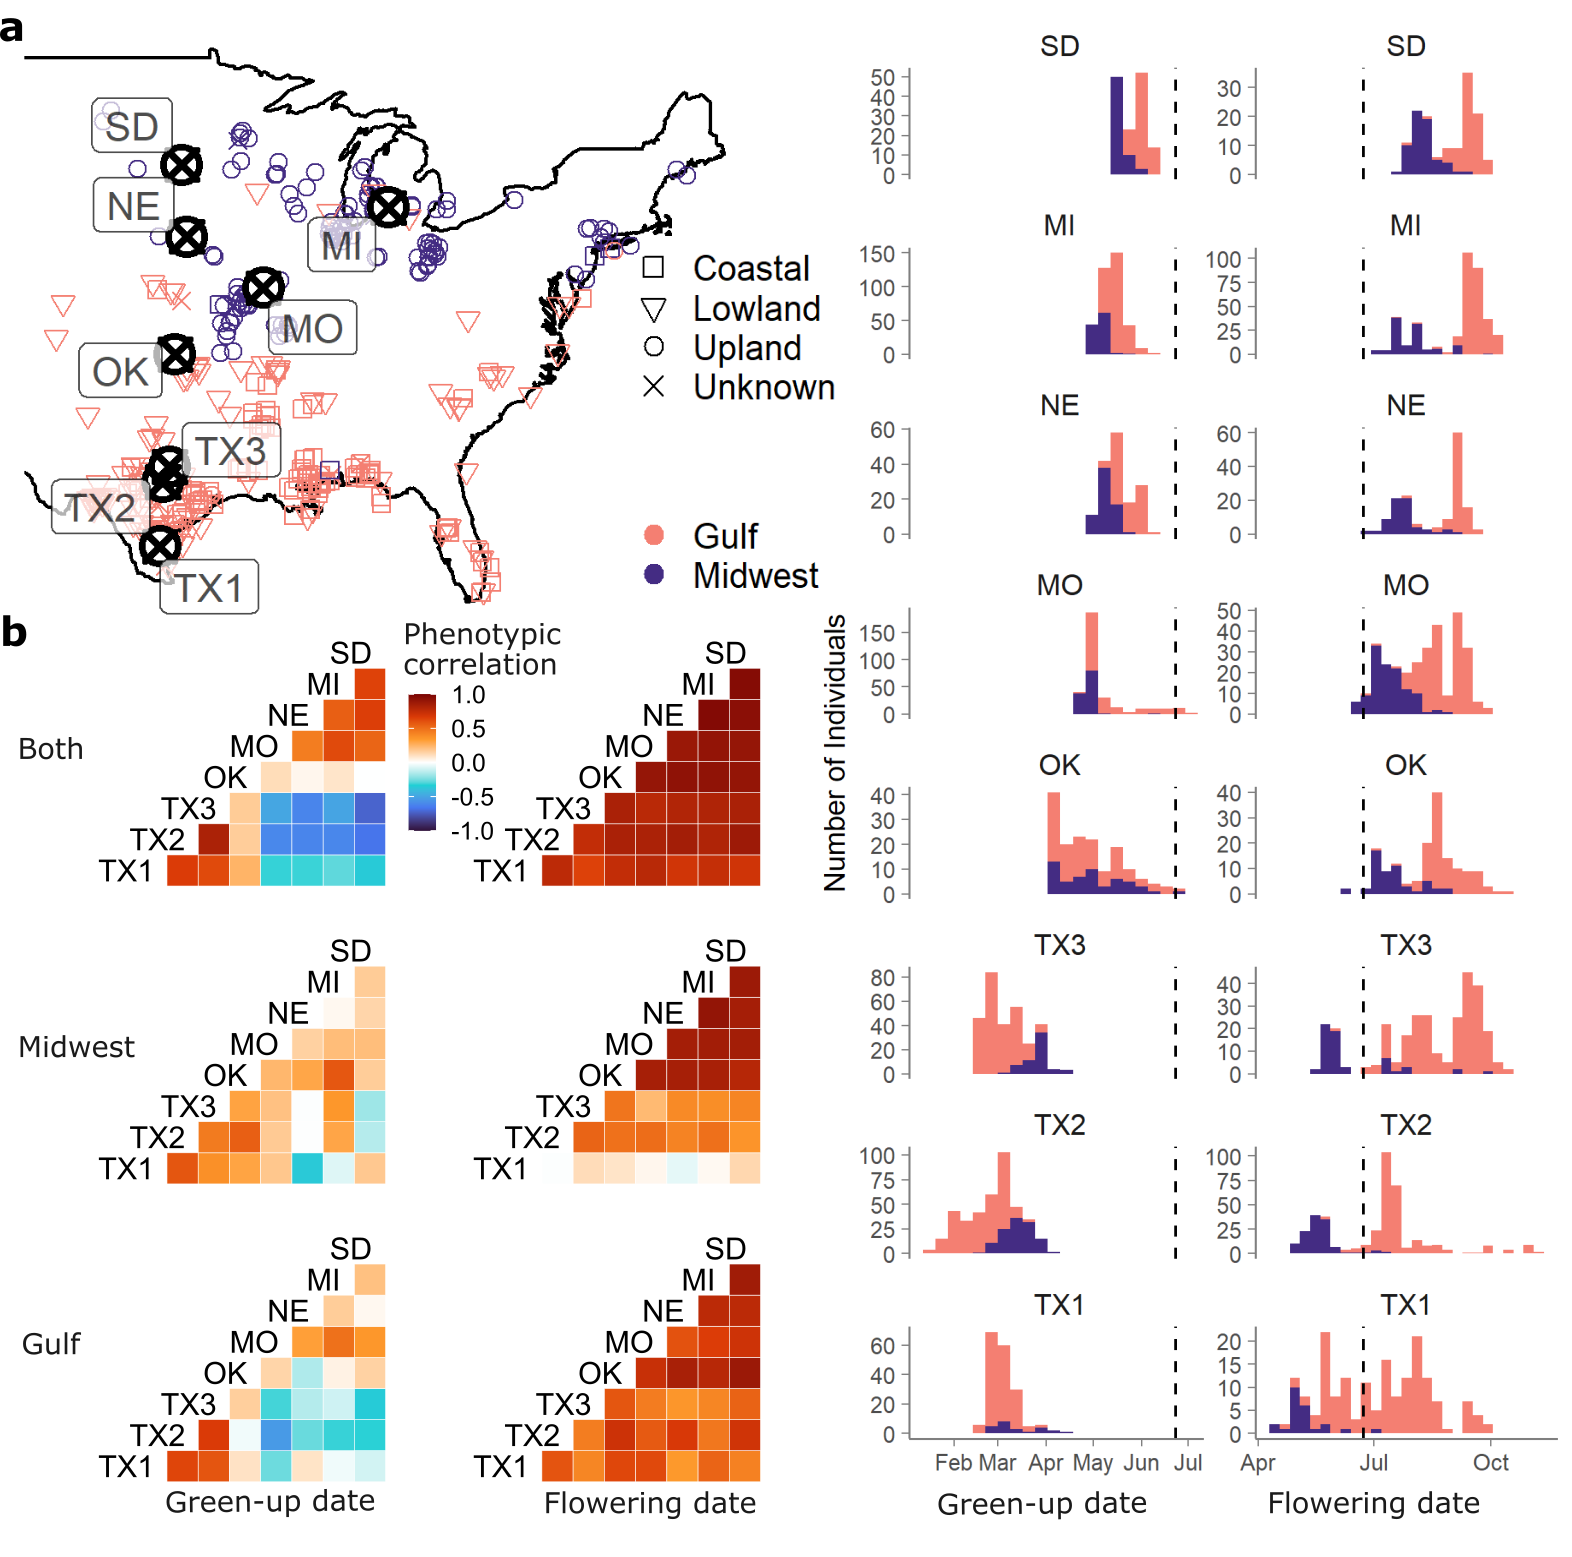
\includegraphics{images/Figure_1_AB.png}

}

\caption{\label{fig-map}Characterization of the timing of the onset of
vegetative (green-up) and reproductive (flowering) growth in the
switchgrass diversity panel. (a) Map and trait histograms of green-up
and flowering dates across two genetically distinct switchgrass
subpopulations and eight common gardens. Purple represents individuals
from the Midwest genetic subpopulation, and pink individuals from the
Gulf subpopulation; map positions represent the original collection
locations for the genotypes, and shapes represent the ecotype of the
genotype. Histogram vertical dashed lines indicate the summer solstice.
Common gardens are arranged in latitudinal order. (b) Phenotypic
correlations between clonal replicates planted at eight common gardens,
within and between two genetic subpopulations.}

\end{figure}%

\begin{figure}

\centering{

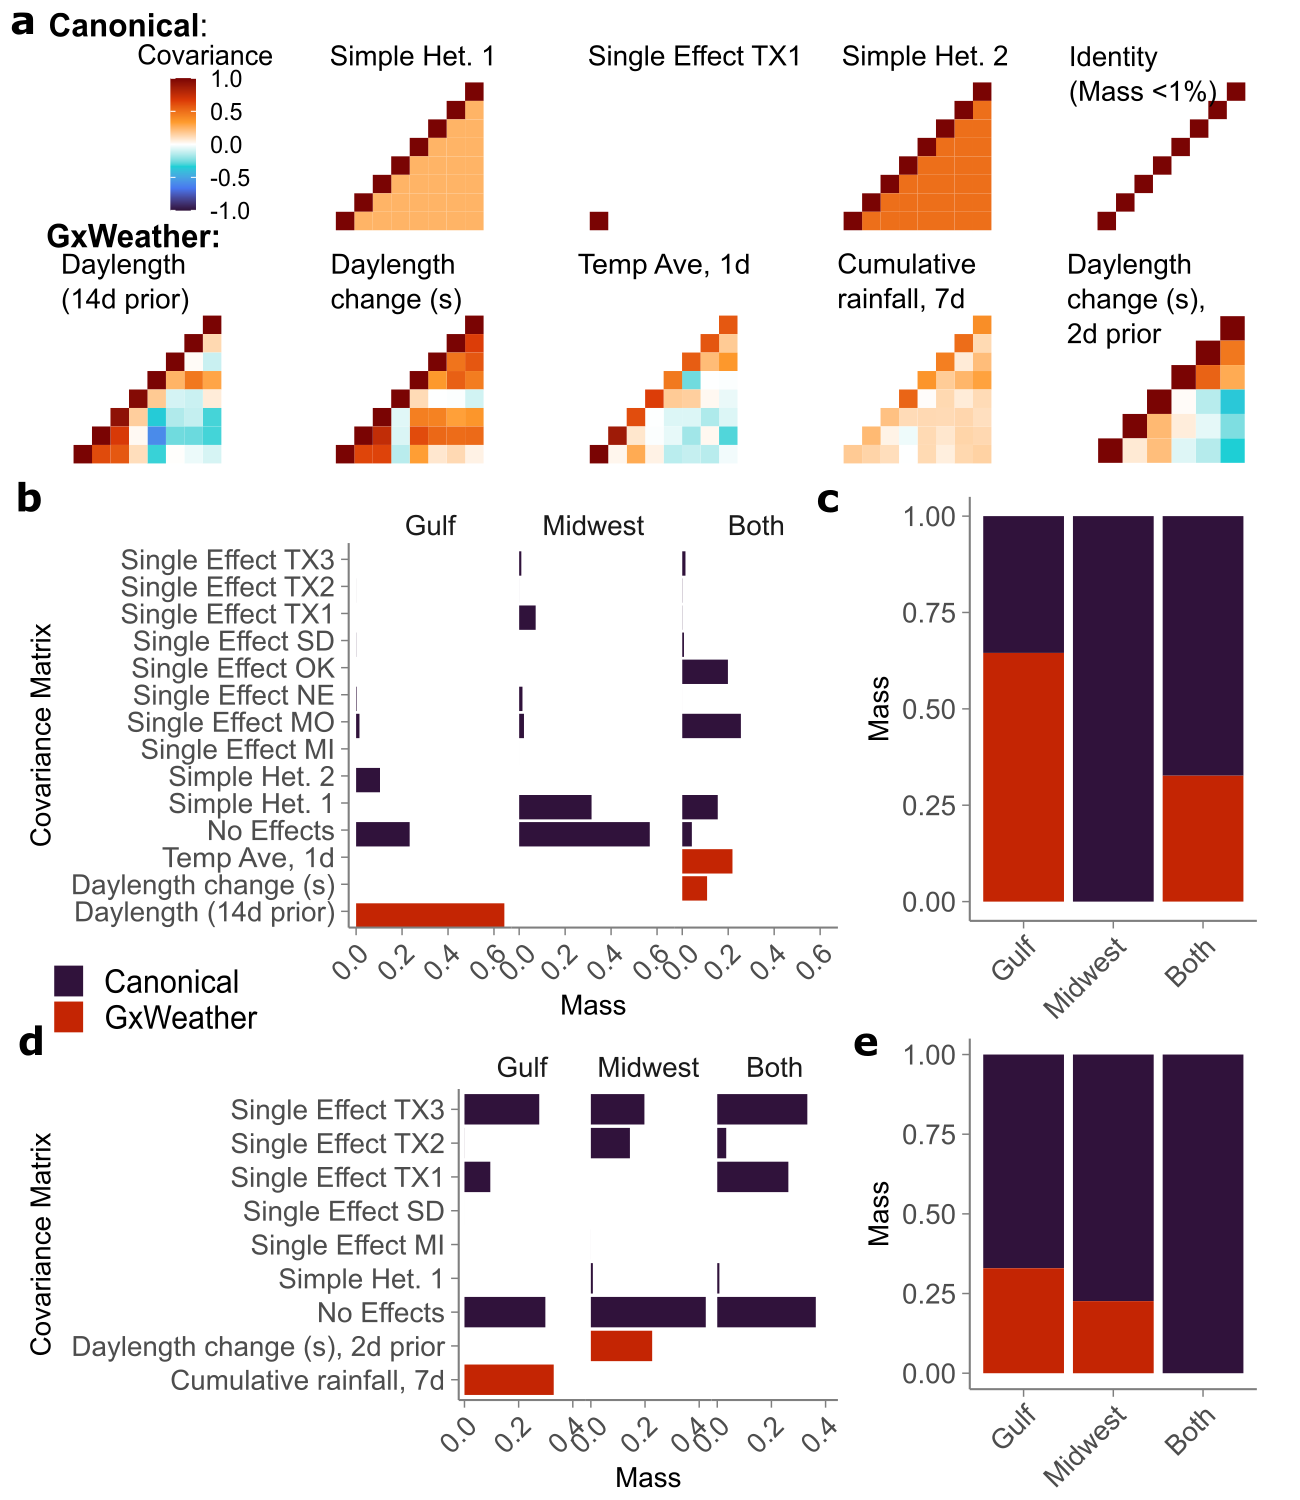
\includegraphics{images/Figure_2.png}

}

\caption{\label{fig-covar}Example hypothesis-driven covariance matrices
specified in \emph{mash} and the posterior weights placed on all
covariance matrices. (a) Common gardens are arranged in latitudinal
order within the matrices. Top row: Four example canonical covariance
matrices. Canonical matrices (purple) have simple interpretations, such
as equal effects across all common gardens, or effects specific to a
single common garden. Bottom row: Five example GxWeather covariance
matrices specified for the green-up date or flowering date phenotype;
these matrices were created from environment-specific correlations
across eight common gardens, and are described in Table 1. (b,d) Total
posterior weight placed on each covariance matrix type specified for (b)
green-up date and (d) flowering date \emph{mash} models, within and
between two genetic subpopulations. Covariance matrices included in
\emph{mash} that had zero posterior weight in all three \emph{mash} runs
on the genetic subpopulations, such as the identity matrix, are not
shown. (c,e) Total posterior weight placed on covariance matrices that
were hypothesized or canonical, for the (c) green-up date phenotype and
(e) flowering date phenotype.}

\end{figure}%

\begin{figure}

\centering{

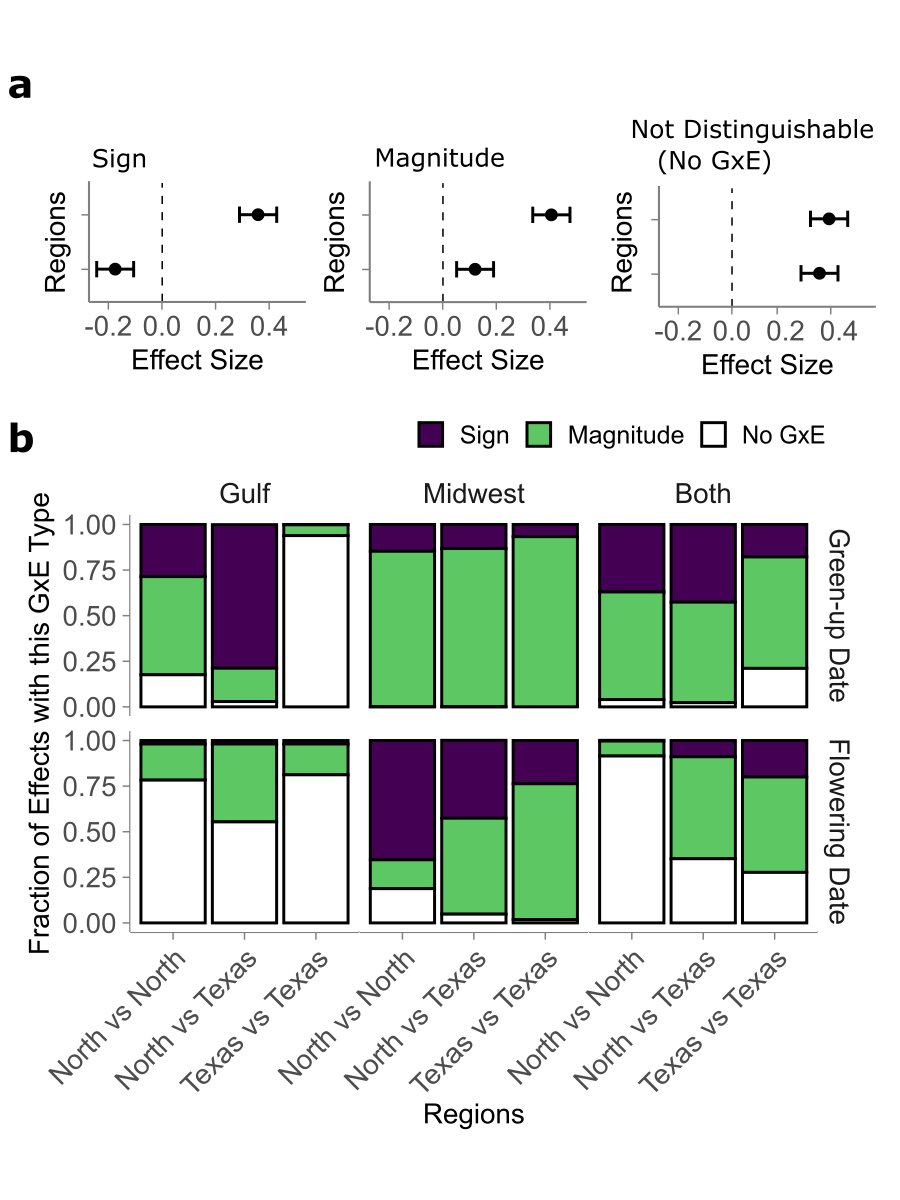
\includegraphics{images/Figure_3_GxE.png}

}

\caption{\label{fig-effects}Types of GxE present between of pairs of
jointly re-estimated effects in eight common gardens, for effects with
lfsr \textless{} 0.05. a) Examples of effect patterns at three pairs of
sites with three types of GxE. All effects are for an alternate allele,
with the reference allele effect defined to be zero at both gardens and
represented by the dashed vertical line. Sign: Effects that differ in
sign at these pairs of gardens (p \textless{} 0.05, lfsr). Magnitude:
Effects identical in sign (p \textless{} 0.05, lfsr) that differ in
magnitude by a factor of \textgreater0.4. Not Distinguishable: Effects
not distinguishable by magnitude nor sign of the effect, with no
measurable GxE. b) The fraction of effects with each GxE type for the
onset of vegetative growth (green-up date) and reproductive growth
(flowering date), within and between two genetic subpopulations. Common
gardens are grouped by the larger region they came from: North gardens
are within the natural range of the Midwest subpopulation, and include
MO, NE, MI, and SD, while Texas gardens are within the natural range of
the Gulf subpopulation, and include TX1, TX2, and TX3.}

\end{figure}%

\begin{figure}

\centering{

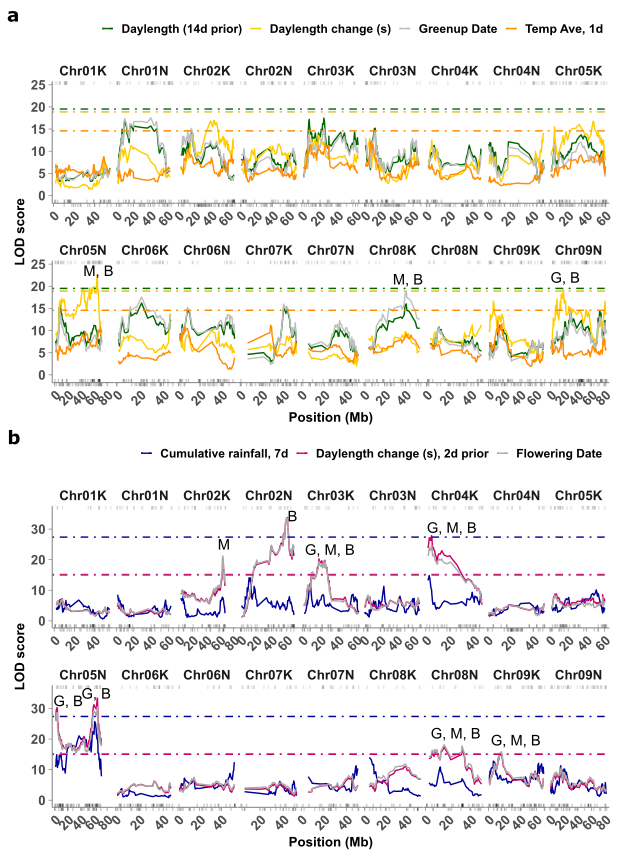
\includegraphics{images/Figure_4_QTL_Overlaps.png}

}

\caption{\label{fig-qtl}Overlaps of QTL from an outbred pseudo-F2 cross
and with jointly re-estimated SNP effects in the 1\% tail of
significance from a diversity panel. Dotted lines indicate
permutation-based significance thresholds for each weather-related
function. Stars indicate QTL with significant enrichment for SNPs in the
1\% \emph{mash} tail; G, M, and B indicate which subpopulation had
enrichment: G - Gulf subpopulation, M -Midwest subpopulation, B - both
subpopulations. Rug plots show genomic locations of SNPs in the 1\%
\emph{mash} tail for flowering date for each subpopulation: Both
subpopulations are above the plot panel, the Gulf subpopulation is above
the x-axis, and the Midwest subpopulation is below the x-axis. a) QTL
mapping for the onset of vegetative growth (green-up date), and three
weather-related functions of green-up date. b) QTL mapping for the onset
of reproductive growth (flowering date), and two weather-related
functions of flowering date.}

\end{figure}%

\section{Materials and Methods}\label{materials-and-methods}

Whenever possible, plant material will be shared upon request. Source
data and code to replicate these analyses are available at:
https://github.com/Alice-MacQueen/pvdiv-phenology-gxe.git. SNP data to
replicate these analyses are available from the UT dataverse at
\url{https://doi.org/10.18738/T8/A604BU}.

\subsection{Scoring onset of vegetative and reproductive development in
two mapping
panels}\label{scoring-onset-of-vegetative-and-reproductive-development-in-two-mapping-panels}

In 2019, we scored two phenological events every two days in two mapping
populations of switchgrass, a diversity panel and a pseudo-F2 cross,
planted at eight common garden locations (35, 40, 41). We scored the
onset of vegetative growth, or green-up date, as the day of the year
when 50\% of the tiller area of the crown of the plant cut the previous
year had green growth. The onset of reproductive growth, or flowering
date, was the day of the year when 50\% of the plant tillers had
panicles undergoing anthesis.

The formation and resequencing of the diversity panel has been described
previously (33). The diversity panel contained 134 sequenced, clonally
propagated individuals from the Midwest genetic subpopulation, and 229
from the Gulf genetic subpopulation. To allow for the possibility that
different subpopulations had different strengths of connection between
our phenotypes and genotypes (42), we conducted three sets of genetic
analyses: on Gulf and Midwest genotypes separately, and on both
subpopulations together (`Both' subpopulations). Analyses to determine
narrow-sense heritability (h\textsuperscript{2}) for green-up and
flowering were done using linear mixed models and followed (33) (SI
Appendix, Section S6).

To confirm candidate genomic regions found using \emph{mash} on the
diversity panel, we analyzed flowering in an outbred pseudo-F2 cross
between four individuals, two Midwest and two Gulf individuals. The
formation of this mapping population has been described previously (35);
additional details on QTL mapping can be found in SI Appendix, Section
S7. To be directly comparable to the diversity panel data, only 2019
phenology data from the pseudo-F2 cross from the same eight common
garden sites were used.

\subsection{Joint re-estimation of SNP effects to assess the frequency
of rank-changing GxE and assignment of genome-wide patterns of GxE and
GxWeather}\label{joint-re-estimation-of-snp-effects-to-assess-the-frequency-of-rank-changing-gxe-and-assignment-of-genome-wide-patterns-of-gxe-and-gxweather}

We were interested in specifying genetic models for trait variation that
allowed more than one form of GxE, as we reasoned that different loci
should display different forms of GxE. In addition, we were interested
in an unbiased estimation of the frequency of rank-changing GxE relative
to other forms of GxE, as the presence of rank-changing GxE at the level
of individual loci is a key theoretical prediction of local adaptation.
\emph{Mash} allowed us to both specify multiple forms of GxE and
GxWeather and conduct unbiased statistical tests for when SNP effects
changed sign between common gardens.

To use \emph{mash} on our diversity panel, we had to specify both a
relatively uncorrelated set of covariance matrices, which in our case
defined types of GxE and GxWeather between gardens, and we had to
specify subsets of SNP effect estimates and standard errors for our
traits at each common garden. To specify a set of covariance matrices,
we first defined many covariance matrices, including GxWeather matrices
that represented the correlation in weather cues between gardenes before
the phenological event (SI Appendix, Section S1), then implemented a
model selection approach that used a greedy algorithm to evaluate if the
log likelihood of the \emph{mash} model was significantly improved as
additional covariance matrices were included (SI Appendix, Section S4).
To specify subsets of SNP effect estimates and standard errors to use
for both the greedy algorithm and with the optimal set of covariance
matrices, we first calculated best linear unbiased predictors (BLUPs)
for each phenological trait in each genetic subpopulation and each
common garden (SI Appendix, Section S2). Next, we determined effect
estimates for 8.8 to 12.3 million SNPs per subpopulation by conducting
garden-specific GWAS on these BLUPs using \(k\) vectors of singular
values to correct for population structure, where \(k\) was the smallest
integer value that made the genomic control coefficient closest to 1 (SI
Appendix, Section S2). Singular values were computed using singular
value decomposition of the matrix of all SNPs, with iterative SNP
pruning and removal of regions in long-range linkage disequilibrium
(43). Third, to make the \emph{mash} models computationally feasible, we
extracted two subsets of SNP effect estimates and standard errors from
our GWAS effect estimates: (i) effects from a subset of ``strong'' tests
corresponding to stronger effects on our traits; (ii) results from a
random subset of all tests to correspond to an unbiased representation
of all effects (SI Appendix, Section S3). We used the subset of random
effects in our greedy \emph{mash} algorithm (SI Appendix, Section S4)
and used the subset of strong effects in our \emph{mash} models with the
optimal set of covariance matrices (SI Appendix, Section S5).

The loadings of genetic effects onto the multiple covariance structures
specified in our \emph{mash} models provided information on genome-wide
patterns of SNP-environment interaction. In addition, the the GxWeather
covariance structures allowed hypothesis testing of specific weather
variables as cues for the start of vegetative and reproductive growth.
Say that a SNP in the gene Flowering Locus C (FLC), a well-known
flowering time regulator, controls flowering in a photoperiod-dependent
manner. In that case, the joint estimate of effects for that SNP could
have a high mixture proportion, or mass, on a covariance matrix created
using a photoperiod-based environmental cue, such as day length at some
interval prior to flowering. In our data, we would infer that the effect
of that SNP on flowering was caused by a response to the environmental
cue used to construct the GxWeather covariance structure with the
largest mass.

Our joint re-estimation of SNP effects also allowed us to characterize
the overall patterns of GxE in the set of SNPs where there was pairwise
significance of effects at pairs of gardens. To do this, we used the
`get\_GxE' function of the switchgrassGWAS R package. First, this
function determines the set of SNPs with evidence of significant effects
in both conditions for all pairs of conditions using local false sign
rates (lfsr) as the significance criteria. Then, this function
determines if effects significant in both conditions are of opposite
sign.

Using the lfsr rather than the local false discovery rate (lfdr) is a
critical change in our ability to detect alleles directly contributing
to rank-changing GxE between environments. The lfdr, like other measures
of FDR, focuses on if we have enough evidence to reject the null
hypothesis that an effect j is 0, or that there is a significant effect.
Previous studies of antagonistic pleiotropy (e.g. (40)) have used the
lfdr or equivalent statistical tests to detect antagonistic pleiotropy.
These tests were conservative, in that they required two non-zero
effects of different signs, while tests for differential sensitivity
required only one non-zero effect. This previous work recognized that
this testing bias could lead to undercounting occurrences of
antagonistic pleiotropy (27, 29), and sought to reduce it by permutation
(28). However, using the lfsr to test for allelic effects that differ in
sign does not undercount these occurences, as this statistic answers a
fundamentally different question. For each effect \(j\), the \(lfsr_j\)
is defined as the probability that we make an error in the sign of
effect \(j\) if we were forced to declare the effect positive or
negative (37). Thus, rather than asking ``Are these two effects
different?'' - as we reasonably expect two effects to be, even if this
difference cannot be measured - the local false sign rate answers a more
meaningful question: Can we be confident in the sign of this effect?

In addition, the get\_GxE function also sets an arbitrary threshold to
count an effect as changing in magnitude between environments, commonly
known as differential sensitivity or a change in amplitude of the
effect. For differential sensitivity, this function determines if
effects significant in both conditions are of the same sign and of a
magnitude (not tested for significance) that differs by a factor of 0.4
or more. The remaining effects that are significant in both conditions
have the same effect sign and similar effect magnitudes and we denote
these effects as having no GxE. The distinction between effects with
different magnitudes is arbitrary but useful to fully characterize how
effects vary across environments to ultimately influence phenotypes. Our
use of the lfsr to determine significance and our specification that SNP
effects must be significant in both conditions to be included means that
our tests for alleles with rank-changing GxE carry an equal statistical
burden to those measuring differential sensitivity and effects without
GxE.

\section{References}\label{references}

\bibsplit[2]

\phantomsection\label{refs}
\begin{CSLReferences}{0}{1}
\bibitem[\citeproctext]{ref-bauerle_photoperiodic_2012}
\CSLLeftMargin{1. }%
\CSLRightInline{W. L. Bauerle, \emph{et al.},
\href{https://doi.org/10.1073/pnas.1119131109}{Photoperiodic regulation
of the seasonal pattern of photosynthetic capacity and the implications
for carbon cycling}. \emph{Proceedings of the National Academy of
Sciences} \textbf{109}, 8612--8617 (2012).}

\bibitem[\citeproctext]{ref-andres2012genetic}
\CSLLeftMargin{2. }%
\CSLRightInline{F. Andrés, G. Coupland, The genetic basis of flowering
responses to seasonal cues. \emph{Nature Reviews Genetics} \textbf{13},
627--639 (2012).}

\bibitem[\citeproctext]{ref-korner2010phenology}
\CSLLeftMargin{3. }%
\CSLRightInline{C. Körner, D. Basler, Phenology under global warming.
\emph{Science} \textbf{327}, 1461--1462 (2010).}

\bibitem[\citeproctext]{ref-botero2015evolutionary}
\CSLLeftMargin{4. }%
\CSLRightInline{C. A. Botero, F. J. Weissing, J. Wright, D. R.
Rubenstein, Evolutionary tipping points in the capacity to adapt to
environmental change. \emph{Proceedings of the National Academy of
Sciences} \textbf{112}, 184--189 (2015).}

\bibitem[\citeproctext]{ref-blackman2013interacting}
\CSLLeftMargin{5. }%
\CSLRightInline{B. K. Blackman, Interacting duplications, fluctuating
selection, and convergence: The complex dynamics of flowering time
evolution during sunflower domestication. \emph{Journal of experimental
botany} \textbf{64}, 421--431 (2013).}

\bibitem[\citeproctext]{ref-henry2014transitions}
\CSLLeftMargin{6. }%
\CSLRightInline{L. P. Henry, R. H. Watson, B. K. Blackman, Transitions
in photoperiodic flowering are common and involve few loci in wild
sunflowers (helianthus; asteraceae). \emph{American Journal of Botany}
\textbf{101}, 1748--1758 (2014).}

\bibitem[\citeproctext]{ref-aagren2017adaptive}
\CSLLeftMargin{7. }%
\CSLRightInline{J. Ågren, C. G. Oakley, S. Lundemo, D. W. Schemske,
Adaptive divergence in flowering time among natural populations of
arabidopsis thaliana: Estimates of selection and QTL mapping.
\emph{Evolution} \textbf{71}, 550--564 (2017).}

\bibitem[\citeproctext]{ref-brachi2010linkage}
\CSLLeftMargin{8. }%
\CSLRightInline{B. Brachi, \emph{et al.}, Linkage and association
mapping of arabidopsis thaliana flowering time in nature. \emph{PLoS
genetics} \textbf{6}, e1000940 (2010).}

\bibitem[\citeproctext]{ref-dittmar2014flowering}
\CSLLeftMargin{9. }%
\CSLRightInline{E. L. Dittmar, C. G. Oakley, J. Ågren, D. W. Schemske,
Flowering time QTL in natural populations of arabidopsis thaliana and
implications for their adaptive value. \emph{Molecular ecology}
\textbf{23}, 4291--4303 (2014).}

\bibitem[\citeproctext]{ref-li2018genomic}
\CSLLeftMargin{10. }%
\CSLRightInline{X. Li, T. Guo, Q. Mu, X. Li, J. Yu, Genomic and
environmental determinants and their interplay underlying phenotypic
plasticity. \emph{Proceedings of the National Academy of Sciences}
\textbf{115}, 6679--6684 (2018).}

\bibitem[\citeproctext]{ref-romero2017study}
\CSLLeftMargin{11. }%
\CSLRightInline{J. A. Romero Navarro, \emph{et al.}, A study of allelic
diversity underlying flowering-time adaptation in maize landraces.
\emph{Nature genetics} \textbf{49}, 476--480 (2017).}

\bibitem[\citeproctext]{ref-wadgymar2017identifying}
\CSLLeftMargin{12. }%
\CSLRightInline{S. M. Wadgymar, \emph{et al.}, Identifying targets and
agents of selection: Innovative methods to evaluate the processes that
contribute to local adaptation. \emph{Methods in Ecology and Evolution}
\textbf{8}, 738--749 (2017).}

\bibitem[\citeproctext]{ref-blumel2015flowering}
\CSLLeftMargin{13. }%
\CSLRightInline{M. Blümel, N. Dally, C. Jung, Flowering time regulation
in crops---what did we learn from arabidopsis? \emph{Current opinion in
biotechnology} \textbf{32}, 121--129 (2015).}

\bibitem[\citeproctext]{ref-jung2009flowering}
\CSLLeftMargin{14. }%
\CSLRightInline{C. Jung, A. E. Müller, Flowering time control and
applications in plant breeding. \emph{Trends in plant science}
\textbf{14}, 563--573 (2009).}

\bibitem[\citeproctext]{ref-turner2005pseudo}
\CSLLeftMargin{15. }%
\CSLRightInline{A. Turner, J. Beales, S. Faure, R. P. Dunford, D. A.
Laurie, The pseudo-response regulator ppd-H1 provides adaptation to
photoperiod in barley. \emph{Science} \textbf{310}, 1031--1034 (2005).}

\bibitem[\citeproctext]{ref-faure2012mutation}
\CSLLeftMargin{16. }%
\CSLRightInline{S. Faure, \emph{et al.}, Mutation at the circadian clock
gene EARLY MATURITY 8 adapts domesticated barley (hordeum vulgare) to
short growing seasons. \emph{Proceedings of the National Academy of
Sciences} \textbf{109}, 8328--8333 (2012).}

\bibitem[\citeproctext]{ref-hung2012zmcct}
\CSLLeftMargin{17. }%
\CSLRightInline{H.-Y. Hung, \emph{et al.}, ZmCCT and the genetic basis
of day-length adaptation underlying the postdomestication spread of
maize. \emph{Proceedings of the National Academy of Sciences}
\textbf{109}, E1913--E1921 (2012).}

\bibitem[\citeproctext]{ref-zakhrabekova2012induced}
\CSLLeftMargin{18. }%
\CSLRightInline{S. Zakhrabekova, \emph{et al.}, Induced mutations in
circadian clock regulator mat-a facilitated short-season adaptation and
range extension in cultivated barley. \emph{Proceedings of the National
Academy of Sciences} \textbf{109}, 4326--4331 (2012).}

\bibitem[\citeproctext]{ref-yang2013oself3}
\CSLLeftMargin{19. }%
\CSLRightInline{Y. Yang, Q. Peng, G.-X. Chen, X.-H. Li, C.-Y. Wu, OsELF3
is involved in circadian clock regulation for promoting flowering under
long-day conditions in rice. \emph{Molecular Plant} \textbf{6}, 202--215
(2013).}

\bibitem[\citeproctext]{ref-pin2012multifaceted}
\CSLLeftMargin{20. }%
\CSLRightInline{P. Pin, O. Nilsson, The multifaceted roles of FLOWERING
LOCUS t in plant development. \emph{Plant, cell \& environment}
\textbf{35}, 1742--1755 (2012).}

\bibitem[\citeproctext]{ref-weller2019parallel}
\CSLLeftMargin{21. }%
\CSLRightInline{J. L. Weller, \emph{et al.}, Parallel origins of
photoperiod adaptation following dual domestications of common bean.
\emph{Journal of Experimental Botany} \textbf{70}, 1209--1219 (2019).}

\bibitem[\citeproctext]{ref-Weine2023.06.21.545998}
\CSLLeftMargin{22. }%
\CSLRightInline{E. Weine, S. P. Smith, R. K. Knowlton, A. Harpak,
Tradeoffs in modeling context dependency in complex trait genetics.
\emph{bioRxiv} (2024)
https:/doi.org/\href{https://doi.org/10.1101/2023.06.21.545998}{10.1101/2023.06.21.545998}.}

\bibitem[\citeproctext]{ref-levene1953genetic}
\CSLLeftMargin{23. }%
\CSLRightInline{H. Levene, Genetic equilibrium when more than one
ecological niche is available. \emph{The American Naturalist}
\textbf{87}, 331--333 (1953).}

\bibitem[\citeproctext]{ref-felsenstein1976theoretical}
\CSLLeftMargin{24. }%
\CSLRightInline{J. Felsenstein, The theoretical population genetics of
variable selection and migration. \emph{Annual review of genetics}
\textbf{10}, 253--280 (1976).}

\bibitem[\citeproctext]{ref-kawecki2004conceptual}
\CSLLeftMargin{25. }%
\CSLRightInline{T. J. Kawecki, D. Ebert, Conceptual issues in local
adaptation. \emph{Ecology letters} \textbf{7}, 1225--1241 (2004).}

\bibitem[\citeproctext]{ref-hedrick1986genetic}
\CSLLeftMargin{26. }%
\CSLRightInline{P. W. Hedrick, Genetic polymorphism in heterogeneous
environments: A decade later. \emph{Annual review of ecology and
systematics} \textbf{17}, 535--566 (1986).}

\bibitem[\citeproctext]{ref-des2013genotype}
\CSLLeftMargin{27. }%
\CSLRightInline{D. L. Des Marais, K. M. Hernandez, T. E. Juenger,
Genotype-by-environment interaction and plasticity: Exploring genomic
responses of plants to the abiotic environment. \emph{Annual Review of
Ecology, Evolution, and Systematics} \textbf{44}, 5--29 (2013).}

\bibitem[\citeproctext]{ref-anderson2013genetic}
\CSLLeftMargin{28. }%
\CSLRightInline{J. T. Anderson, C.-R. Lee, C. A. Rushworth, R. I.
Colautti, T. Mitchell-Olds, Genetic trade-offs and conditional
neutrality contribute to local adaptation. \emph{Molecular ecology}
\textbf{22}, 699--708 (2013).}

\bibitem[\citeproctext]{ref-anderson2011evolutionary}
\CSLLeftMargin{29. }%
\CSLRightInline{J. T. Anderson, J. H. Willis, T. Mitchell-Olds,
Evolutionary genetics of plant adaptation. \emph{Trends in Genetics}
\textbf{27}, 258--266 (2011).}

\bibitem[\citeproctext]{ref-mitchell1997predicting}
\CSLLeftMargin{30. }%
\CSLRightInline{R. B. Mitchell, K. J. Moore, L. E. Moser, J. O. Fritz,
D. D. Redfearn, Predicting developmental morphology in switchgrass and
big bluestem. \emph{Agronomy Journal} \textbf{89}, 827--832 (1997).}

\bibitem[\citeproctext]{ref-parrish2005biology}
\CSLLeftMargin{31. }%
\CSLRightInline{D. J. Parrish, J. H. Fike, The biology and agronomy of
switchgrass for biofuels. \emph{BPTS} \textbf{24}, 423--459 (2005).}

\bibitem[\citeproctext]{ref-casler2004latitudinal}
\CSLLeftMargin{32. }%
\CSLRightInline{M. Casler, K. P. Vogel, C. Taliaferro, R. Wynia,
Latitudinal adaptation of switchgrass populations. \emph{Crop Science}
\textbf{44}, 293--303 (2004).}

\bibitem[\citeproctext]{ref-lovell2021genomic}
\CSLLeftMargin{33. }%
\CSLRightInline{J. T. Lovell, \emph{et al.}, Genomic mechanisms of
climate adaptation in polyploid bioenergy switchgrass. \emph{Nature}
\textbf{590}, 438--444 (2021).}

\bibitem[\citeproctext]{ref-porter1966analysis}
\CSLLeftMargin{34. }%
\CSLRightInline{C. L. Porter Jr, An analysis of variation between upland
and lowland switchgrass, panicum virgatum l., in central oklahoma.
\emph{Ecology} \textbf{47}, 980--992 (1966).}

\bibitem[\citeproctext]{ref-milano2016genetic}
\CSLLeftMargin{35. }%
\CSLRightInline{E. R. Milano, D. B. Lowry, T. E. Juenger, The genetic
basis of upland/lowland ecotype divergence in switchgrass (panicum
virgatum). \emph{G3: Genes, Genomes, Genetics} \textbf{6}, 3561--3570
(2016).}

\bibitem[\citeproctext]{ref-urbut2019flexible}
\CSLLeftMargin{36. }%
\CSLRightInline{S. M. Urbut, G. Wang, P. Carbonetto, M. Stephens,
Flexible statistical methods for estimating and testing effects in
genomic studies with multiple conditions. \emph{Nature genetics}
\textbf{51}, 187--195 (2019).}

\bibitem[\citeproctext]{ref-10.1093ux2fbiostatisticsux2fkxw041}
\CSLLeftMargin{37. }%
\CSLRightInline{M. Stephens,
\href{https://doi.org/10.1093/biostatistics/kxw041}{{False discovery
rates: a new deal}}. \emph{Biostatistics} \textbf{18}, 275--294 (2016).}

\bibitem[\citeproctext]{ref-choi2023}
\CSLLeftMargin{38. }%
\CSLRightInline{S. Choi, \emph{et al.},
\href{https://doi.org/10.1093/jxb/erad255}{A single amino acid change
led to structural and functional differentiation of {\emph{PvHd1}} to
control flowering in switchgrass}. \emph{Journal of Experimental Botany}
\textbf{74}, 5532--5546 (2023).}

\bibitem[\citeproctext]{ref-savolainen2013ecological}
\CSLLeftMargin{39. }%
\CSLRightInline{O. Savolainen, M. Lascoux, J. Merilä, Ecological
genomics of local adaptation. \emph{Nature Reviews Genetics}
\textbf{14}, 807--820 (2013).}

\bibitem[\citeproctext]{ref-lowry2019qtl}
\CSLLeftMargin{40. }%
\CSLRightInline{D. B. Lowry, \emph{et al.}, QTL\(\times\) environment
interactions underlie adaptive divergence in switchgrass across a large
latitudinal gradient. \emph{Proceedings of the National Academy of
Sciences} \textbf{116}, 12933--12941 (2019).}

\bibitem[\citeproctext]{ref-lovell2021}
\CSLLeftMargin{41. }%
\CSLRightInline{J. T. Lovell, \emph{et al.},
\href{https://doi.org/10.1038/s41586-020-03127-1}{Genomic mechanisms of
climate adaptation in polyploid bioenergy switchgrass}. \emph{Nature},
1--7 (2021).}

\bibitem[\citeproctext]{ref-kortefarlow2013}
\CSLLeftMargin{42. }%
\CSLRightInline{A. Korte, A. Farlow, The advantages and limitations of
trait analysis with GWAS: A review. \emph{Plant methods} \textbf{9}, 29
(2013).}

\bibitem[\citeproctext]{ref-privuxe92017}
\CSLLeftMargin{43. }%
\CSLRightInline{F. Privé, H. Aschard, M. G. B. Blum,
\href{http://dx.doi.org/10.1101/190926}{Efficient management and
analysis of large-scale genome-wide data with two r packages: Bigstatsr
and bigsnpr} (2017).}

\end{CSLReferences}

\acknow{We thank the Brackenridge Field laboratory, the Ladybird Johnson
Wildflower Center, and the Juenger laboratory for support with plant
care and propagation. This material is based upon work supported in part
by the Great Lakes Bioenergy Research Center, U.S. Department of Energy,
Office of Science, Office of Biological and Environmental Research under
Award Numbers DE-SC0018409 and DE-FC02-07ER64494, the US Department of
Energy Awards DESC0014156 to T.E.J., DE-SC0017883 to D.B.L, National
Science Foundation PGRP Awards IOS0922457 and IOS1444533 to T.E.J, and
the Long-term Ecological Research Program (DEB 1832042) at the Kellogg
Biological Station.}

\showacknow{} % Display the acknowledgments section


\end{document}
